\documentclass[11pt]{article}

\usepackage[margin=1in]{geometry}


\usepackage[dvipsnames]{xcolor}
\newcommand{\rev}[1]{{\color{RoyalBlue}#1}}

% use proper unicode fonts
\usepackage[T1]{fontenc}
\usepackage[utf8]{inputenc}
\usepackage{fixltx2e}

\usepackage{amsmath} % for better display of equations

\usepackage{setspace}
\usepackage{natbib} 

\usepackage{titling} % controls the way the title information is displayed
\pretitle{\begin{flushleft}\Large}
\posttitle{\end{flushleft}}
\predate{}
\postdate{}
\preauthor{\begin{flushleft}}
\postauthor{\end{flushleft}}
\setlength{\droptitle}{-3em}

\usepackage{authblk} % adds some nice options for displaying the author list
\renewcommand\Authsep{\protect\\}
\renewcommand\Authands{\protect\\}

%% graphics packages
\usepackage{graphicx}
\usepackage[nomarkers, tablesfirst]{endfloat} % for final
\usepackage{caption}
\captionsetup{labelsep=none,textformat=empty} % for final
% \captionsetup{labelformat=simple} % for drafts
\usepackage{booktabs}
\usepackage{multirow}


\usepackage{lineno}

%% ----------------------------------
%
%     Packages to be used for drafts and editing
%     Remove from the final manuscript
%
%% ----------------------------------
%\usepackage[top=1in, left=1in, bottom=1in, right=2.0in]{geometry}
%\usepackage[textsize=tiny, backgroundcolor=white, textwidth=1.8in, colorinlistoftodos=true]{todonotes} % for margin notes using \todo{}
%\newcommand{\mt}[1]{\todo[color=blue!40]{\textsuperscript{MT}#1}}
%\newcommand{\ib}[1]{\todo[color=red!40]{\textsuperscript{IB}#1}}
%\newcommand{\fd}[1]{\todo[color=orange!40]{\textsuperscript{FD}#1}}
%\newcommand{\dg}[1]{\todo[color=green!40]{\textsuperscript{DG}#1}}


%% ----------------------------------
%
%     Title and authorship information
%
%% ----------------------------------


\title{Cross-scale integration of knowledge for predicting species ranges: a metamodeling framework}
\date{}
\author[1,2,13]{Matthew V. Talluto (mtalluto@gmail.com)}
\author[1,2]{Isabelle Boulangeat (isabelle.boulangeat@gmail.com)}
\author[3]{Aitor Ameztegui (ameztegui@gmail.com)}
\author[4]{Isabelle Aubin (Isabelle.Aubin@NRCan-RNCan.gc.ca)}
\author[1,2,5]{Dominique Berteaux (Dominique\_Berteaux@uqar.ca)}
\author[1,2]{Alyssa Butler (ca.butler10@gmail.com)} 
\author[6,7]{Frédérik Doyon (Frederik.Doyon@uqo.ca)}
\author[8]{C. Ronnie Drever (cdrever@tnc.org)}
\author[9]{Marie-Josée Fortin (mariejosee.fortin@utoronto.ca)}
\author[1]{Tony Franceschini (Tony.Franceschini@uqar.ca)}
\author[10]{Jean Liénard (jean.lienard@gmail.com)}
\author[4]{Dan McKenney (Dan.McKenney@nrcan-rncan.gc.ca)}
\author[2,3]{Kevin A. Solarik (kevinsolarik@hotmail.com)}
\author[10]{Nikolay Strigul (nick.strigul@vancouver.wsu.edu)}
\author[11,12]{Wilfried Thuiller (wilfried.thuiller@ujf-grenoble.fr)}
\author[1,2]{Dominique Gravel (dominique\_gravel@uqar.ca)}
\affil[1]{Département de biologie, Université du Québec à Rimouski, Rimouski, Quebec, Canada}
\affil[2]{Quebec Centre for Biodiversity Science, Montreal, Quebec, Canada}
\affil[3]{Centre d'Étude de la Forêt, Département des sciences biologiques, Université du Québec à Montréal, Montreal, Quebec, Canada}
\affil[4]{Great Lakes Forestry Centre, Canadian Forest Service, Natural Resources Canada, Sault Ste Marie, Ontario, Canada}
\affil[5]{Centre for Northern Studies, Université du Québec à Rimouski, Rimouski, Quebec, Canada}
\affil[6]{Université du Québec en Outaouais, Gatineau, Quebec, Canada}
\affil[7]{Institut des Sciences de la Forêt Tempérée (ISFORT), Ripon, Quebec, Canada}
\affil[8]{The Nature Conservancy Canada, Ottawa, Ontario, Canada}
\affil[9]{Department of Ecology and Evolutionary Biology, University of Toronto, Toronto, Ontario, Canada}
\affil[10]{Department of Mathematics, Washington State University, Vancouver, Washington, USA}
\affil[11]{Université Grenoble Alpes, Laboratoire d’Ecologie Alpine (LECA), F-38000 Grenoble, France}
\affil[12]{CNRS, Laboratoire d’Ecologie Alpine (LECA), F-38000 Grenoble, France}
\affil[13]{Author for correspondance. Address: Departament de Biologie, chimie, et geographie, 300, Allée des Ursulines, Rimouski, Quebec G5L 3A1, Canada}


%% ----------------------------------
%
%     END PREAMBLE
%
%% ----------------------------------

\begin{document}
\doublespacing
%% ----------------------------------
%
%     TITLE PAGE
%
%% ----------------------------------

%TC:ignore
\begin{titlingpage}
	\maketitle
	
	\begin{flushleft}
	
	\textbf{Short title:} Integrated models of species ranges
	
	\textbf{Abstract word count: } 235 %ABS_COUNT
	
	\textbf{Main text word count: } 5083 %WORD_COUNT %Target 5000
	
%	\textbf{Authorship:} All authors contributed substantially to an initial outline of the paper and ideas. MT, IB, and DG built the model and wrote the first draft of the introduction and model description. All authors contributed to the complete first draft and all subsequent revisions to the manuscript.
		
	\textbf{Keywords:} Climate change, decision making, patterns and processes, range dynamics, scaling, spatial ecology, species distribution modeling, uncertainty
	\end{flushleft}
\end{titlingpage}
%TC:endignore

%TC:break abstract
\linenumbers
\begin{abstract}
\noindent

Current interest in forecasting potential changes to species ranges have resulted in a great diversity of approaches to species distribution modeling.
However, in general, single approaches include only a small subset of the available information about a species. 
Correlative models often predict presence or absence as a function of the environment, but ignore smaller-scale processes such as growth, fecundity, and dispersal.
Furthermore, different approaches often produce divergent predictions, with no simple method to reconcile them.
We present a flexible framework for integrating models at multiple scales using hierarchical Bayesian methods. 
Our framework uses a metamodel, estimated in a hierarchical Bayesian framework, that is constrained by both data directly applied to the metamodel and by the results of one or more sub-models.
The output of the metamodel is in the form of probabilistic estimates of species presence.
Metamodel outputs also incorporate uncertainty from both data and process error from all sub-models, and include all of the information used as input for the original scale-specific sub-models.
We illustrate our approach using theoretical and empirical examples, and demonstrate that the framework better characterizes uncertainty and can substantially reduce it when projecting beyond the range of the original data.
We conclude by discussing the application of our method and its accessibility to conservation biologists and land managers.
The framework has wide potential for use in species distribution modelling, and can drive better integration of multi-scale data into ecological decision-making.

 \end{abstract}

%TC:break manuscript
%% ----------------------------------
%
%     INTRODUCTION
%
%% ----------------------------------

\section*{Introduction}

Models of species range limits have wide applications and can play a large role in conservation biology, where they can be used as decision-support tools in biodiversity management \citep{Guisan2013}.
Due to large temporal and spatial scales as well as the complex and nonlinear nature of ecosystem dynamics, it is often impossible to construct experiments that can adequately explore the ecological processes generating species range limits \citep{Wu1995, Levin1998}. 
Hence, range models are essential tools that have been applied to a large number of ecological subfields, including biogeography \citep{Schurr2012}, invasion biology \citep{Catterall2012, Gallien2012}, hybrid zone dynamics \citep{Engler2013}, and climate change impacts on species distributions \citep{Blois2013, Thuiller2014}. 

Despite the recognized potential of these models, it can be difficult to produce species distribution models (SDMs) with acceptable levels of precision and bias \citep{Guisan2013}.
For mechanistic models, two important constraints can cause difficulties: (1) having the appropriate ecological theory needed to link data to modeling objectives, and (2) having sufficient data over a range of conditions to maintain coherence between the spatial and temporal scales of data and theory.
In recent decades, however, modeling techniques have proliferated to take advantage of increased data availability. 
A growing body of theory, reflecting the diversity of processes generating species ranges, also has contributed to model diversification \citep{Boulangeat2012}.
Of these model types, fine-scale mechanistic models may capture important ecological processes quite well, but due to their specificity, perform poorly when applied at the scale of species ranges.
For instance, biotic interactions are usually not modeled mechanistically at the scale of species distributions because they are poorly known or have not been recorded, despite being considered a key determinant of range limits \citep{Pigot2013}. 
In contrast to mechanistic models, more correlative approaches that statistically relate species occurrences to associated distributions of other variables have the advantage of indirectly accounting for all underlying processes \citep{Guisan2000}.
However, their predictions rely on the stationarity of the relationships between occurrences and explanatory variables in time and space, implying that the selected variables are related to the processes limiting species ranges and that their correlations are constant for calibration and projection ranges in space and time \citep{Dormann2007}. 
Extrapolating beyond the scope of the original data (e.g., predicting ranges based on future climate) is therefore problematic, because nonlinearities in responses to novel combinations of the explanatory variables cannot be accommodated in models that do not simulate the underlying processes.
%% ----------------------------------
%% ----------------------------------
%% ----------------------------------

Clearly, an approach is needed to unify the strength of different modeling approaches that can incorporate multiple data sources and modeling paradigms.
Toward this end, we present here an application of hierarchical Bayesian methods that uses outputs from multiple models to inform the results of the final model.
Techniques for multimodel inference have proliferated in recent years.
For example, hybrid models that allow for flexible combinations between mechanistic and phenomenological sub-models are commonly employed in SDMs \citep{Gallien2010, Thuiller2013, Boulangeat2014}.
Within the hybrid framework, a correlative model might be used to account for abiotic variables limiting species distributions \citep{Guisan2005}, while a more mechanistic approach could include biotic interactions and space-time dynamics through dispersal \citep{Smolik2010}.
However, the link between different sub-models is based on assumptions about the scaling of ecological processes that are poorly known and difficult to test \citep{Gallien2010}, uncertainties are approximated and their attribution to different sources is difficult to distinguish.
A commonly-employed alternative to hybrid models is the direct combination of predictions, where predictions from models operating at the same spatio-temporal scales can be combined \citep[e.g., model averaging, ensemble forecasting;][]{Araujo2007}. 
However, the applicability of such techniques is limited; for example, because uncertainty is approximated and may be poorly understood, it is not possible to evaluate the effects of convergent predictions on the total uncertainty of the outcomes, despite its potential importance in a prediction context.

We propose an alternative to these other approaches using a hierarchical Bayesian framework. 
This approach provides a number of desirable advantages, including (1) the ability to incorporate multiple modes of inference (e.g., mechanistic, correlative models) \citep{VanOijen2005, Clark2006, Hobbs2011, Hartig2012}, (2) an easy mechanism to include multiple data sources at various scales \citep{Levin1992, Peters2004}, and (3) an intuitive and comprehensive reporting of uncertainty in model predictions that reflects uncertainty at all levels of organization \citep{Cressie2009, Hobbs2011}.
Contrary to hybrid methods, the aim is not to link different sub-models into a single one, but to condition the predictions of a metamodel at the target scale (e.g., an entire species' range) with information from independent sub-models at a variety of spatial scales, allowing for more flexibility regarding the type of information included. 
By integrating all available knowledge while producing a single prediction, our approach potentially mitigates the limitations inherent in each individual model, contributing to more robust predictions \citep{Guisan2005, Araujo2006}.
Moreover, a more comprehensive understanding of uncertainty can guide biodiversity management and prioritize future data collection by identifying the parameters that contribute most to variance in the model predictions \citep{McMahon2011}. 

We illustrate our framework with two examples.
We begin with a hypothetical example, using simulated data, where we define the framework and demonstrate its application to multiple sources of information from different scales.
In a second example, we apply the framework to combine presence-absence information with phenological data to improve uncertainty estimates and reduce bias when predicting changes to the range of sugar maple (\emph{Acer saccharum} Marsh.), a widespread and dominant tree species from eastern North America, in response to climate change.
We provide a more formal mathematical presentation in Appendix S1, along with complete code and data for both examples (Appendix S2).

%% ----------------------------------
%
%     EXAMPLE 1
%
%% ----------------------------------
\section*{Example 1: Adding experimental evidence for the fundamental niche to a species distribution model}
The key idea of our approach is to formulate a metamodel that integrates data at the same ecological scale as the desired predictions, and to constrain the parameters of this model using the output of one or more sub-models.
In this hypothetical example, we build a metamodel relating the distribution of an annual plant to coarse-scale climate with complementary information originating from a fine-scale experiment manipulating the precipitation regime.
The metamodel attempts to capture the realized distribution of a species; as a correlative model, it implicitly captures the major physiological constraints and ecological processes constraining the distribution of the target species. 
However, for the purposes of forecasting, we would like to disentangle the fundamental response of a species to environmental variation from other processes in order to map the climatic envelope of where a species may be found in a natural setting.
Thus, we use additional information on the physiological constraints affecting species distribution.
Because these data are often collected at a finer scale than that of rangewide occurence data, we apply a simple scaling function, drawing on ecological theory, to compute the likelihood of a set of metamodel parameters given both the occurrence and the physiological data.
See Appendix S1 for procedural details and scripts for executing the model.

%==================
%TC:ignore
\begin{figure}[t]
	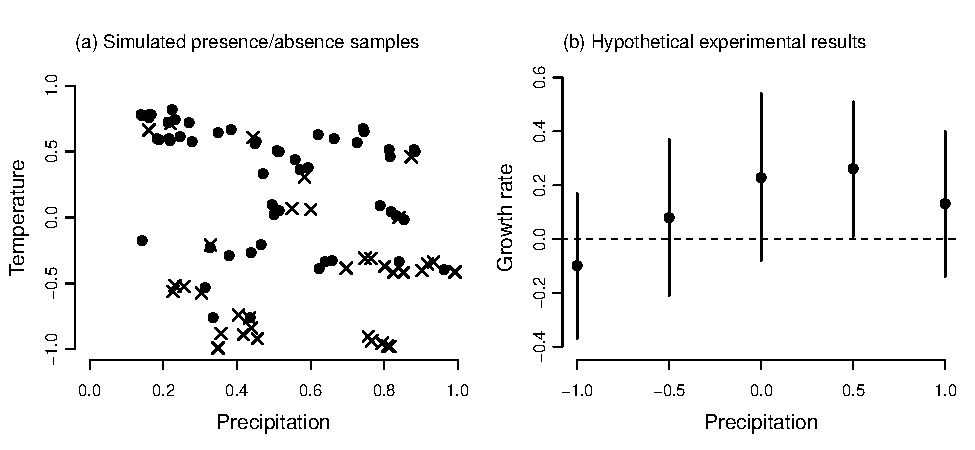
\includegraphics{figs/ex1_sampling.pdf}
	\caption{Two simulated datasets used to illustrate the model integration framework.
	(a) Presences (circles) or absences (x's) of the species in ecological space, \rev{where the range of precipitation values sampled was 0.1--1}.
	(b) Growth rate ($r$) as a function of manipulations to the precipitation regime (whiskers show $\pm$ 1 SE), with a larger range for precipitation (i.e., -1.0--1.0).
	The dashed line shows the threshold above which the species net growth rate is positive (implying presence).
	Axis scales for temperature and precipitation are arbitrary, but note the different scales on the horizontal axes.}
	\label{fig:ex1_sampling}
\end{figure}
%TC:endignore
%==================

We consider data collected from a species' historical distribution, where the goal is to predict the distribution following a substantial reduction in precipitation.
For the metamodel-scale data, we simulate a relatively high-quality presence-absence dataset covering a variety of ecological conditions, which we term \(X_M\), where the subscripted \(M\) indicates that the data were collected at the same scale as the metamodel (Fig. \ref{fig:ex1_sampling}).
We desire to model the species' distribution as a function of temperature, \(T_M\), and precipitation, \(P_M\).
An initial version of the metamodel \((\theta_M)\) that has no constraints from other datasets will be referred to as the naive model.
This naive model uses a simple logistic regression to estimate the naive probability of occurrence \((\psi_N)\) as a function of second order effects of temperature and precipitation:

%-----
\begin{equation}
\begin{aligned}
	\psi_N &= f\left(\theta_M, T_M, P_M \right) \\
	&= p \left (X_M = 1 \mid \theta_M, T_M, P_M \right) \\
	&=\text{logit}^{-1}\left( \theta_M D_M \right)
\end{aligned}
\end{equation}
%-----
where \(\theta_M\) is the parameter vector of the model, \(D_M\) is the covariate matrix (i.e., \(T_M, P_M\)), and \(\text{logit}^{-1}\) is the inverse of the logit function.
We estimate parameters using a Metropolis-Hastings algorithm within a Markov Chain Monte Carlo (MCMC) method using the proportional form of Bayes' theorem:

%-----
\begin{equation}
\label{eq:ex1_bayes}
	p\left (\theta_M \mid X_M,T_M,P_M \right ) \propto 
	p \left(X_M \mid \theta_M, T_M, P_M \right)
	p \left(\theta_M \right)
\end{equation}
%-----
where \(p\left(X_M \mid \theta_M, T_M, P_M \right)\) is often referred to as the \emph{likelihood} of the data (\(X_M\)) given the model (\(\theta_M\)), \(p\left(\theta_M \right)\) is often referred to as the \emph{prior distribution} of \(\theta_M\), and the goal of modeling is to estimate \(p\left (\theta_M \mid X_M,T_M,P_M \right )\), the \emph{posterior distribution} of \(\theta_M\), which gives the probability that \(\theta_M\) takes particular values, given the observed data.

Thus far, we have considered only a single source of information to fit this model, and therefore the prior distribution \(p\left(\theta_M \right)\) from Eq. \ref{eq:ex1_bayes} is uninformative.
As a secondary source of information, we will consider an experiment relating the population growth rate of the plant to manipulations to the precipitation regime, with results (but no raw data) available from the literature (Fig. \ref{fig:ex1_sampling}b). 
Furthermore, no information is available regarding the temperature regime for the experiment.
Transplant experiments that evaluate performance beyond the range of a species are common, and represent a plausible scenario for model integration \citep{Hargreaves2014}.
According to niche theory \citep{Holt2009}, the fundamental niche corresponds to the set of environmental conditions where the per capita intrinsic growth rate $r$ is positive.
This concept gives us a reasonable model to fit a scaling function for our sub-model (Appendix S1).
If we hypothesize that the errors from Figure \ref{fig:ex1_sampling}b \( \left(\sigma_{S} \right) \) are normally distributed (where the \(S\) subscript indicates information pertaining to the submodel), then for an observation $i$, we can interpret the probability of presence \( \left(\psi_{S,i}\right)\) as the probability that the observed growth rate \(X_{S,i}\) is positive:
\begin{equation}
	\psi_{S,i} = \int_0^\infty N \left(X_{S,i}, \sigma_{S,i} \right)
\end{equation}
where \(N\) is the normal density function.
We can then estimate the posterior distribution for the sub-model by fitting the relationship between \(\psi_S\) and precipitation \( \left( P_S \right) \) using Bayesian beta regression \citep{Ferrari2004}:
%-----
\begin{equation}
\label{eq:ex1_thetas}
	p\left (\theta_S \mid \psi_S,P_S \right ) \propto 
	p \left(\psi_S \mid \theta_S, P_S \right)
	p \left(\theta_S \right) \\
\end{equation}
%-----

Although the two datasets were collected at considerably different scales, we have sub-model predictions arising from a fine-scale experiment that are relevant at the scale of the metamodel (i.e., the probability of presence at a given precipitation). 
The scaling treats the fundamental niche as the only driver of species distribution, and only considers a single dimension of the niche.
As such, it would be unwise to expect predictions from this model alone to resemble the actual distribution of the species; as a mechanistic model, it is simply too incomplete to predict distribution.
However, the information from this sub-model, when applied as a constraint on the metamodel, can result in improved predictions that incorporate the information within each model.

We accomplish model integration by treating \(\psi_S\), the posterior predictions of the submodel \(\theta_S\), as prior information about some of the parameters of \(\theta_M\) (i.e., parameters related to precipitation), expanding Equation \ref{eq:ex1_bayes} to incorporate the new information from the sub-model:
%-----
\begin{equation}
	\label{eq:ex1_integrated}
	\overbrace{p(\theta_M \mid X_M, T_M, P_M, \theta_S, \psi_S)}^\text{integrated posterior}
	\propto
	\overbrace{p\left (\psi_S \mid \theta_M,P_M \right )}^{\substack{\text{new information} \\ \text{from sub-model}}}
	\overbrace{p \left(X_M \mid \theta_M, T_M, P_M \right) p \left(\theta_M \right)}^{\substack{\text{naive metamodel} \\ \text{posterior}}}
	\overbrace{p \left(\theta_S \right)}^{\substack{\text{prior for} \\ \text{sub-model}}}	
\end{equation}
%-----
%\dg{There is something wrong with the following equation, or I missed the reasonning somewhere in the last year. In any case, I tried to understand the logic from the text and haven't succeed at it. Either it needs to be fixed, or it needs to be better explained. If I don't get it, my prior tells me nobody will. This equation is central to the paper now that the maths have been put in the appendix. I was expecting to see the likelihood of X\_M given the parameters theta\_M.  The prior of theta\_M being the posterior of the model theta\_M applied to the data psi\_S. The actual likelihood gives the probability of observing the prediction of the sub-model given the parameters of the sub-model. There is not integration on the conditions, it only results from the product of the probabilities.}
As before, the metamodel \(\theta_M\) can be used to predict probability of occurrence \((\psi_I)\).
However, these predictions now reflect the presence-absence data \(X_M\) as well as the information from \(\theta_S\), including all of the data sources used to produce this sub-model.
Finally, we note the presence of marginal distributions for both models (i.e., \(p(\theta_M)\) and \(p(\theta_S)\)).
These can be informative (e.g., incorporating further prior information or the predictions of additional sub-models), semi-informative (e.g., to provide greater weight to more informative models), or uninformative.
For purposes of this example, we applied prior weights of 1 and 0.05 to the correlative and mechanistic models, respectively, reflecting the increased generality and much larger sample size of the correlative data.
This procedure has the effect of increasing the variance of the model and prevents biasing the parameter estimation in favor of the mechanistic model.

%==================
\begin{figure}[bt]
	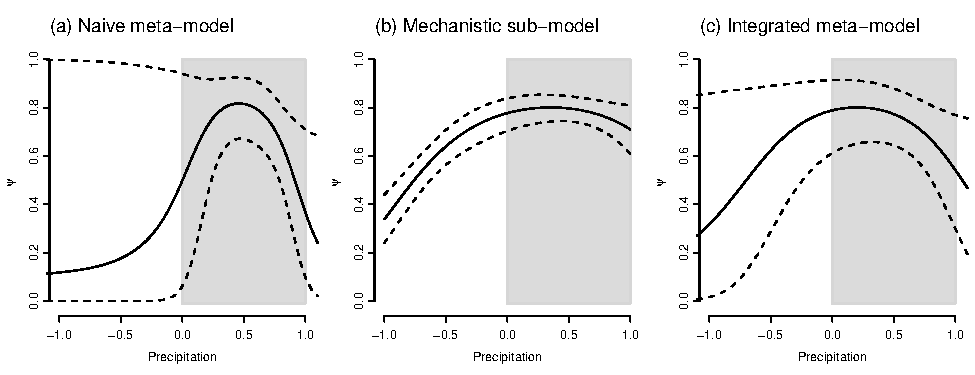
\includegraphics{figs/ex1_precip.pdf}
	\caption{Comparison of the naive model, mechanistic sub-model, and the integrated model showing the probability of presence $(\psi)$ as a function of precipitation.
	Uncertainty is represented as dashed lines, showing the limits of 90\% Bayesian credible intervals.
	The shaded region shows the calibration range for the naive model.
	(a) Naive model, using only presence-absence data. Uncertainty increases dramatically when attempting to project beyond the scope of the source data.
	(b) Mechanistic model, using observations of an experiment to infer probability of presence.
	(c) Integrated model, showing predictions that are intermediate between the two sub-models and uncertainty that is reduced compared to (a).
	}
	\label{fig:ex1_precip}
\end{figure}
%==================


%==================
\begin{figure}[tb]
	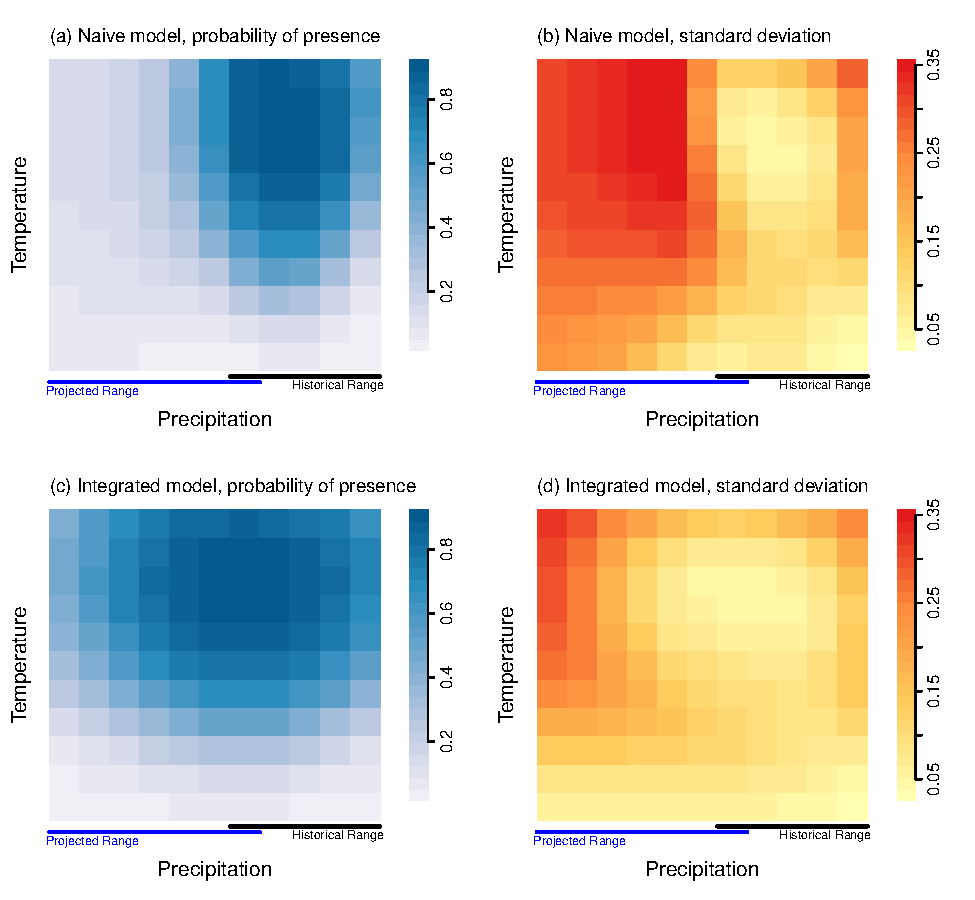
\includegraphics[width=5.25in]{figs/ex1_map.pdf}
	\caption{Maps showing the predicted probability of presence (\(\psi\); (a) and (c)) and the standard deviation of \(\psi\) ((b) and (d)) for the naive and integrated models.
	Historical (i.e., where presence-absence samples were available) and predicted future precipitation regimes are shown below the horizontal axes.
}
	\label{fig:ex1_map}
\end{figure}
%==================

When comparing the three models (naive metamodel, mechanistic sub-model, and integrated metamodel), we observed extreme uncertainty in the first model when projecting beyond the range of the original data (Figs. \ref{fig:ex1_precip}a, \ref{fig:ex1_map}a, \ref{fig:ex1_map}b).
The sub-model was highly precise with respect to precipitation, thus providing a fairly strong constraint when producing the integrated model (Fig \ref{fig:ex1_precip}b).
The result was an integrated prediction that reflected the shapes of both models and showed considerably reduced uncertainty (Fig. \ref{fig:ex1_precip}).
At the scale of the metamodel, considering both temperature and precipitation, we observed similar results, with reduced uncertainty in the predictions over the domain not covered by the presence-absence data (Fig. \ref{fig:ex1_map}).


%% ----------------------------------
%
%     EXAMPLE 2
%
%% ----------------------------------


\subsection*{Example 2: Constraining an SDM using phenological information}
For the second example, we consider the problem of forecasting the potential distribution of a species following climate change.
There is considerable interest in comparing correlative and mechanistic projections with respect to climate change \citep{Morin2009}, and correctly characterizing uncertainty is a critical aspect of this problem \citep{Cheaib2012}.
Despite being a relatively common application of SDMs \citep{Guisan2005}, projecting models parameterized with modern climate data to future climate scenarios remains problematic \citep{Araujo2006}.
We used our framework to constrain a climate-based SDM with information obtained from Phenofit, a mechanistic model that predicts a species' probability of presence as a function of the suitability of the environment given the species' phenology \citep{Chuine2001, Morin2009}.
Here we describe briefly the dataset, methods, and the results of the analysis (see \rev{ Appendix S1 for implementation details and Appendix S2} for data and scripts to reproduce the analysis).

We obtained climate variables, occurrence data, and Phenofit projections at 0.5-degree resolution for both the present and for \rev{2100} for sugar maple, an economically and ecologically important species occurring in eastern North America \citep{Morin2009}.
These data defined the metamodel scale.
To these data, we added 4903 recorded presences and 21701 absences derived from permanent forest sample plots located in the United States and Canada (See Appendix S1 for a map of plot locations).
We reserved 1/3 of this dataset for evaluation, and used the remaining records to calibrate the models.
We constructed the naive model by using a binomial generalized linear model (GLM) to relate the presence-absence dataset to three climate variables: the number of degree days (ddeg), mean annual precipitation (an\_prcp), and the ratio of annual precipitation to potential evapotranspiration (pToPET).
These variables were selected from an initial set of \rev{seven} variables \citep[see Appendix S1 and ][for details on the climate variables]{Morin2009}.
We selected a GLM for its simplicity and interpretability because our focus was on demonstrating the framework, but more complex methods (e.g., generalized additive models) are compatible with the framework.

To perform the integration, we constrained the estimates of the naive model with the additional information from Phenofit while considering two different potential modeling goals.
The first is improving our model of the present range of the species.
Using both datasets to develop a range model for the species has a number of advantages.
Assuming we have chosen climate variables that well represent the constraints on the species, including Phenofit in our model is likely to reduce bias in our estimate of the fundamental niche.
The posterior predictions of the model (that is, the probability of presence projected into geographic space) will incorporate uncertainty from all sources, including the modeling process, data, parameterization, and the ecological processes included.
This can provide a much more accurate estimate of the uncertainty of our predictions.
Thus, for our first integration we combined the naive model with the Phenofit predictions for the present; we refer to this model as ``Integrated-Present'' hereafter.
We also validated this model and compared it against the naive model by computing the area under the receiver operating curve (AUC), a commonly-used metric that measures the rate of correct classification and varies from 0 to 1 (where a value of 1 indicates perfect classification and 0.5 indicates no difference from a random model) \citep{Swets1988}.
The second modeling goal is projecting changes to the range of sugar maple following climate change.
Process-based models and correlative models often differ substantially when projecting beyond the range of the original data (see Example 1).
Thus, we obtained predictions for 2100 from Phenofit \citep{Morin2009} and used them to condition the metamodel given the results of the naive model under future climate.
This procedure provided a consensus view of the future range of the species; we refer to this model as ``Integrated-Future.''
\rev{In both cases, it was necessary to scale the Phenofit predictions, which were probabilistic and not directly derived from the macroclimatic variables used in to fit the naive model, to make them compatible with the naive model, which was based on occurrence data.
We used a latent variable approach, where an unobserved occurrence dataset similar to the one used for the naive model was generated at each MCMC iteration by drawing occurrences from a Binomial distribution with probabilities equal to the probability of occurrence from Phenofit (see Appendix S1 for a full statistical presentation of the model).
This has several advantages.
In addition to expressing the information from Phenofit in a way that is compatible with the naive model, the uncertainty in the predictions is automatically propagated (by simulating a new pseudo-dataset at each iteration), and it becomes possible to address future distribution via simulated future occurrences, (which, by nature, are unobservable).}


\begin{table}[t]
	\footnotesize
	\caption{\rev{Parameter estimates and 95\% credible intervals for the naive model (i.e., a species distribution model fit with occurrence data only), and two integrated models combining predictions from the naive model and either the present or future predictions from a mechanistic model. All models were fit on predictor variables standardized to mean=0 and unit variance, and all estimates are on the logit scale. Climate variables included the number of degree days (ddeg), mean annual precipitation (an\_prcp), and the ratio of annual precipitation to potential evapotranspiration (pToPET).}}
	\begin{tabular}{lcccccccc}
	\toprule
	& Naive & Integrated-present & Integrated-future \\
	\midrule
	\multirow{2}{*}{intercept} & -0.886 & -0.103 & -1.037 \\
	& (-1.12, -0.66) & (-0.23, 0.026) & (-1.16,-0.92) \\
	& & & \\
	
	\multirow{2}{*}{ddeg} & 2.904 & 3.701 & 6.431 \\
	& (2.34, 3.45) & (3.37, 4.03) & (6.07, 6.79) \\
	& & & \\
	
	\multirow{2}{*}{ddeg\textsuperscript{2}} & -6.697 & -6.216 & -5.241 \\
	& (-7.04, 6.35) & (-6.43,-6.00) & (-5.43,-5.05) \\
	& & & \\
	
	\multirow{2}{*}{ddeg\textsuperscript{3}} & 1.669 & 1.454 & 0.893 \\
	& (1.52, 1.79) & (1.37, 1.53) & (0.85, 0.94) \\
	& & & \\
	
	\multirow{2}{*}{an\_prcp} & 0.358 & 0.612 & 1.412 \\
	& (-0.26, 1.02) & (0.28, 0.94) & (1.11, 1.71) \\
	& & & \\
	
	\multirow{2}{*}{an\_prcp\textsuperscript{2}} & -0.571 & -0.848 & -0.975 \\
	& (-0.76,-0.40) & (-0.95,-0.75) & (-1.06,-0.90) \\
	& & & \\
	
	\multirow{2}{*}{pToPET} & 2.960 & 2.637 & 2.093 \\
	& (2.29, 3.61) & (2.28, 2.99) & (1.70, 2.48) \\
	& & & \\
	
	\multirow{2}{*}{pToPET\textsuperscript{2}} & -0.557 & -0.093 & 0.0064 \\
	& (-0.74,-0.37) & (-0.15,-0.03) & (-0.070,-0.073) \\
	\bottomrule
	\end{tabular}
	\label{tab:ex2_params}
\end{table}

%==================
\begin{figure}[t]
	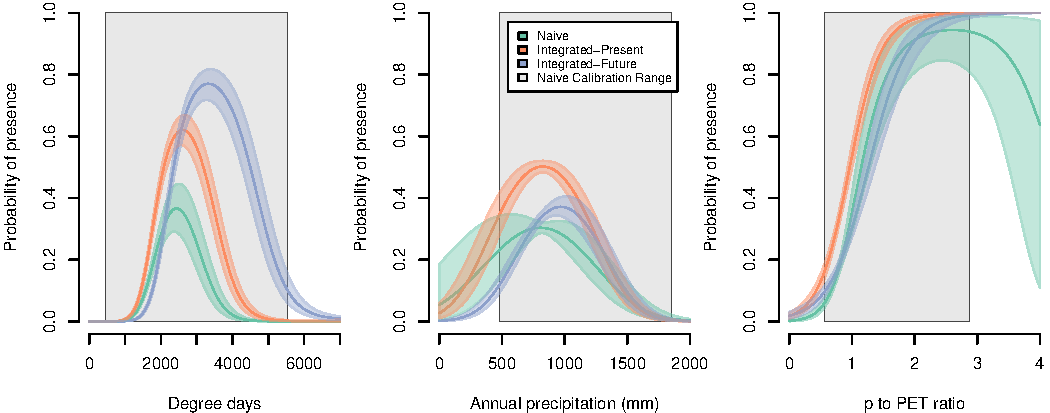
\includegraphics[width=6.5in]{figs/ex2_response.pdf}
	\caption{Response curves for each environmental variable for the three models.
	Predictions are broadly similar for the three models, with an increase the optimal temperature regime predicted by the Integrated-Future model (left panel).
	Integration reduced prediction uncertainty for all three variables, particularly for domains outside the naive calibration range.
	Single-variable predictions were computed with the other variables set to their medians.}
	\label{fig:ex2_response}
\end{figure}
%==================

%==================
\begin{figure}[t]
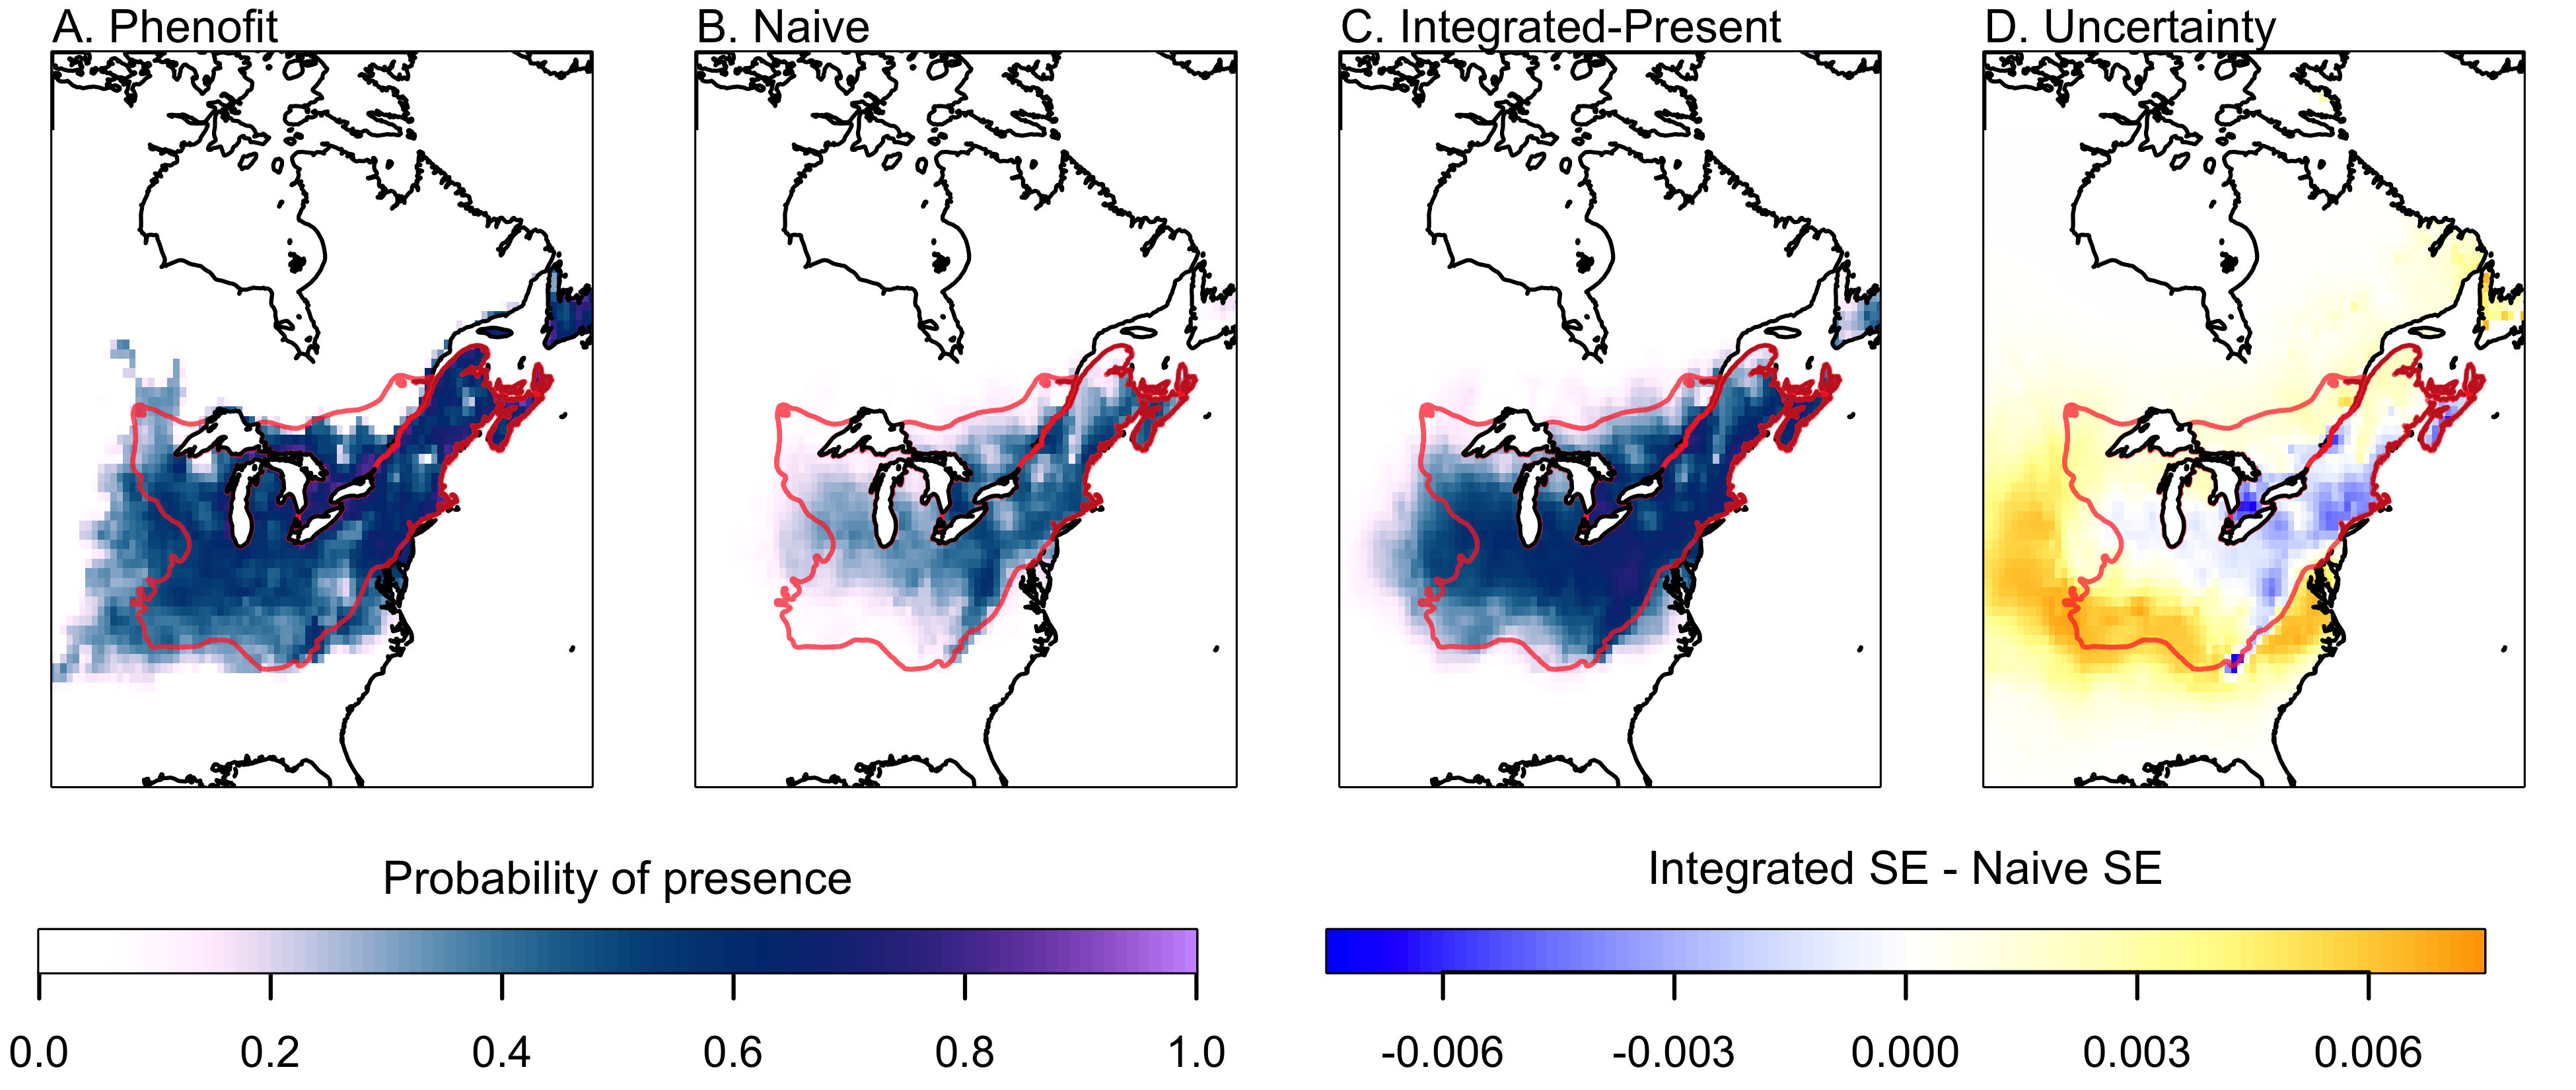
\includegraphics[width=6.5in]{figs/ex2_pres_map.pdf}
\caption{Range predictions for present climate for Phenofit (A), the naive model (B), the Integrated-Present model (C), and the difference between posterior prediction standard errors of the Integrated-Present and Naive models.
Model predictions were quite similar, with reduced uncertainty where the models were in strongest agreement, and increased uncertainty near the range boundary where the models disagreed.
For reference, the present range of the species is outlined in red \citep{Little1971}}.
\label{fig:ex2_map_pres}
\end{figure}

%==================

% results
%% compare parameters
Model integration resulted in substantial reduction in posterior uncertainty in the parameters, and, for the Integrated-Future model, a relatively large revision in the the estimate for the response of sugar maple to temperature (i.e., variable ddeg) (Table \ref{tab:ex2_params}, Fig. \ref{fig:ex2_response}).
When projecting beyond the calibration range for the naive model, the greater coverage provided by the integrated model produced substantial reductions in uncertainty (Fig. \ref{fig:ex2_response}).
When considering the present species distribution, the naive and Integrated-Present models made very similar predictions (Fig. \ref{fig:ex2_map_pres}).
Furthermore, both models performed relatively well when evaluated against reserved data, with AUC values of 0.72 and 0.73 for the naive and integrated models, respectively.
The small difference between the models indicates that both models effectively predict the probability of presence of sugar maple.
The major advantage to integration is the improved understanding of uncertainty in the predictions, with greater uncertainty in southern portions of the range (Fig. \ref{fig:ex2_map_pres}).
It is important to note that the naive model was the basis for the integrated model; thus the increased uncertainty present in the integrated model is not the result of a ``worse'' model, but rather should be viewed as a correction to overfitting in the naive model. 
The uncertainty in the integrated model includes uncertainty arising from the processes that we have incorporated into the metamodel.
Phenofit predicts fitness based on how climate affects phenological timings, frost injury, reproduction, and survival \citep{Chuine2001, Morin2009}.
Thus, climatic factors that ultimately limit species distribution might be quite different under Phenofit, as illustrated by the substantial differences in the potential future distributions predicted by Phenofit and the naive model.


\begin{figure}[t]
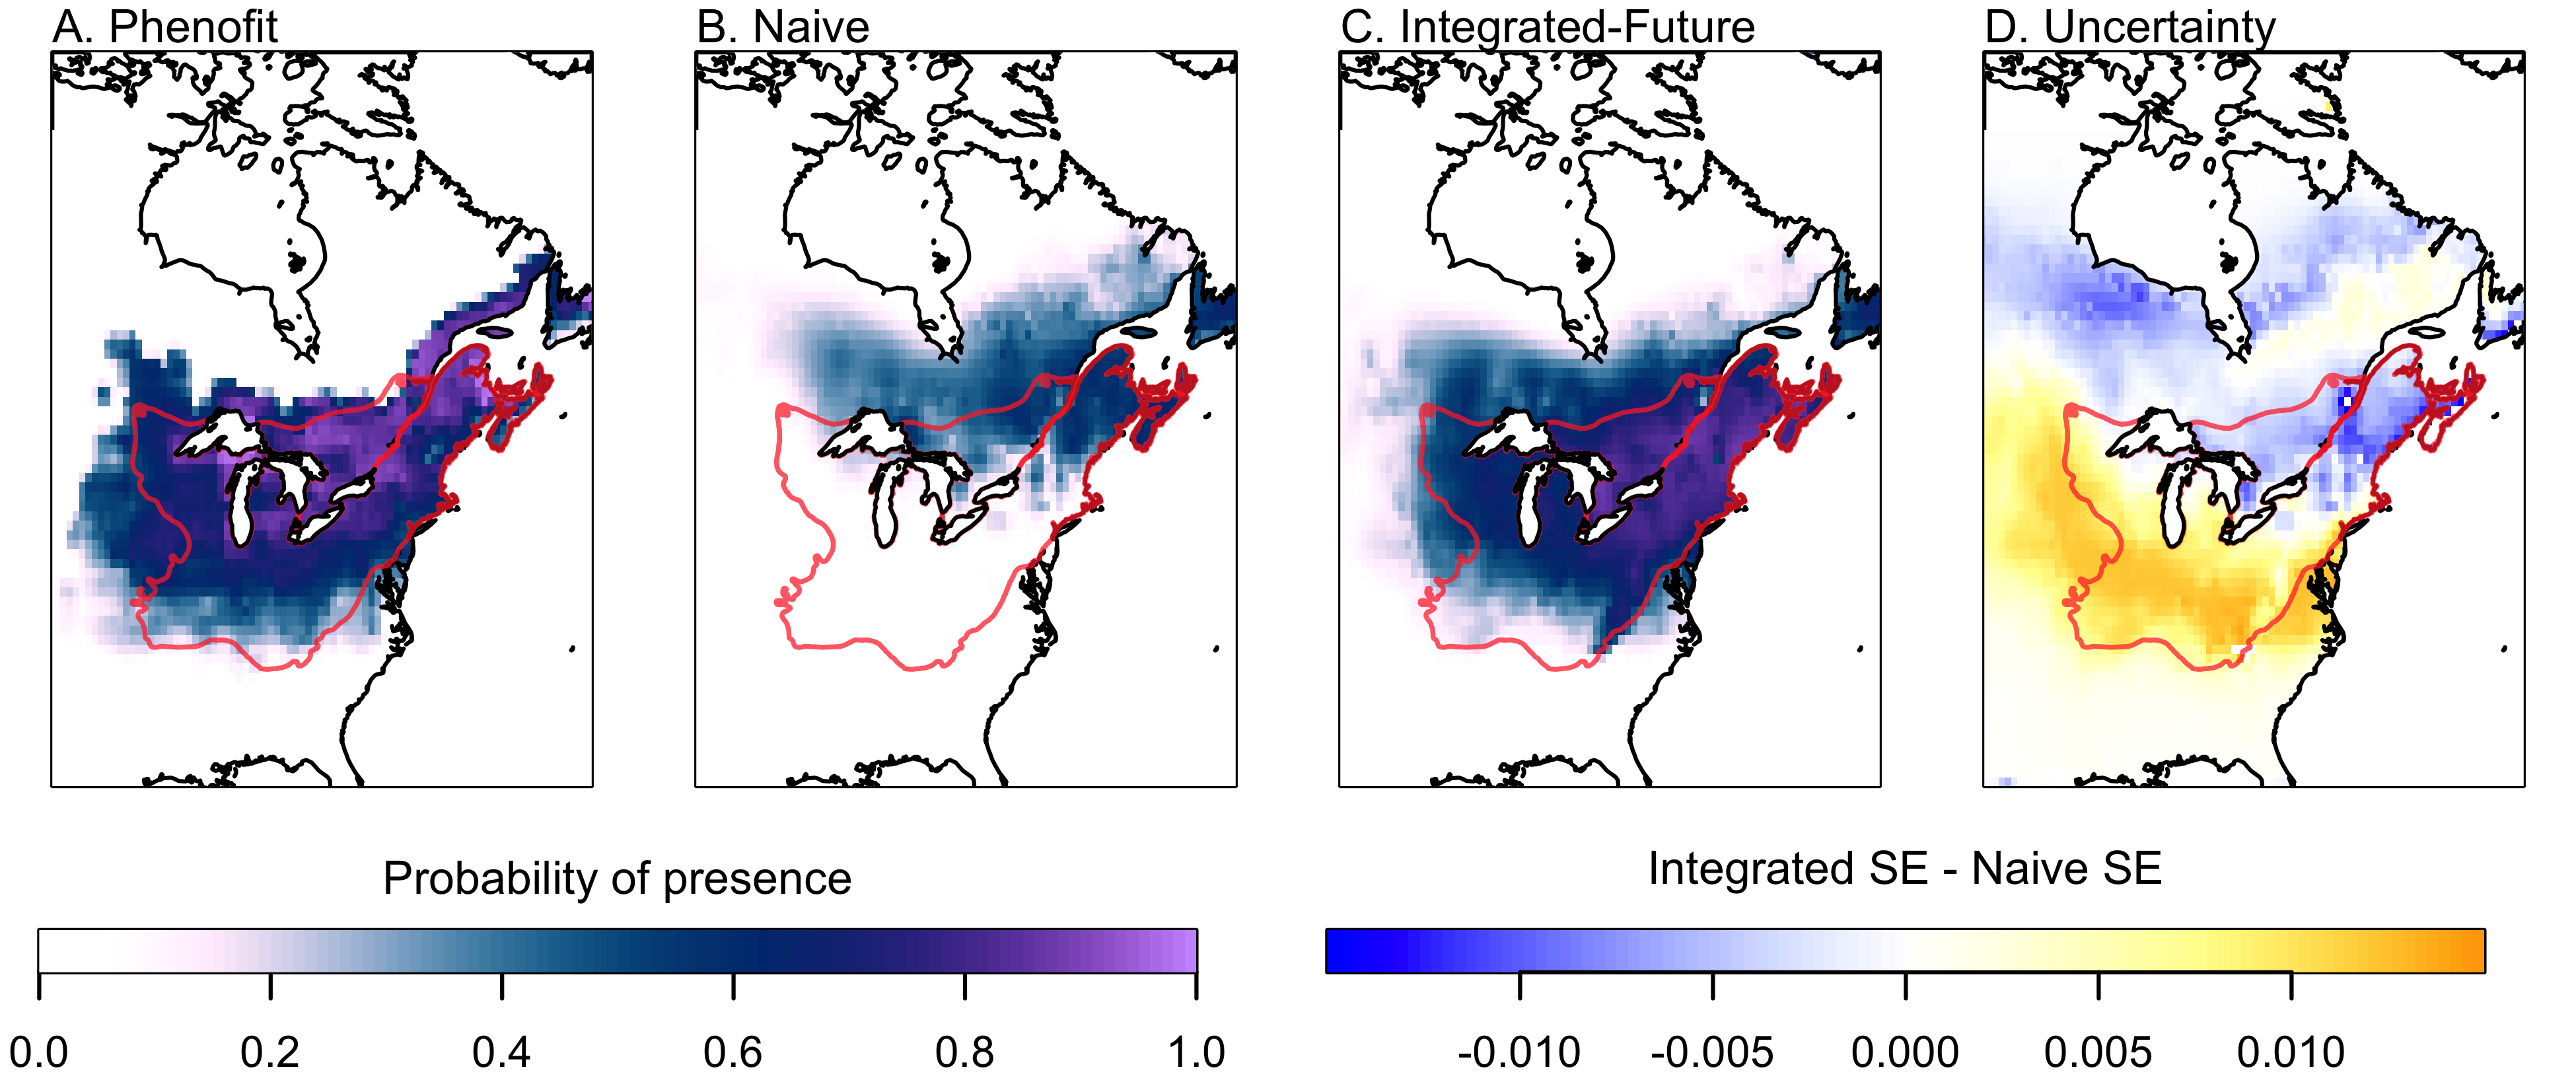
\includegraphics[width=6.5in]{figs/ex2_fut_map.pdf}
\caption{Range predictions for future climate for Phenofit (A), the naive model (B), the Integrated-Future model (C), and the difference between posterior prediction standard errors of the Integrated-Future and Naive models.
The mechanistic sub-model Phenofit (A) predicted small shifts sugar maple range.
In contrast, the naive model (B) projected a large northward change in suitable habitat.
Model integration (C) produced predictions that were intermediate between the two models.
Uncertainty decreased for the northern portion of the present range (red outline) where the models were in agreement, while it increased in the southern portion of the range where the models were in strong disagreement.}
\label{fig:ex2_map_fut}
\end{figure}

The Integrated-Future model presents a different interpretation of the response of sugar maple to warmer temperatures. 
The naive model predicted a substantial northward migration; in other words, the expectation under the naive model \rev{is that the present estimate of the realized niche (obtained using occurrence data) is an unbiased reflection of the fundamental niche; thus the species should track temperature northward as the climate warms}.
The Integrated-Future model, in contrast, predicted substantially more tolerance to warmer temperatures, reflecting similar predictions from Phenofit (Figs. \ref{fig:ex2_response}, \ref{fig:ex2_map_fut}).
\rev{This is because Phenofit estimates different aspects of the realized niche.}
Although both models predicted a northward range shift, the change under Phenofit was limited to approximately 200 km north of the present range limit of the species, compared with more than 900 km for the naive model.
Phenofit also predicted little change in the southern range limit of the species, while the naive model projected loss of the species over much of the southern portion of the range (Fig. \ref{fig:ex2_map_fut}).
\rev{The metamodel thus presents a consensus view of the niche of the species with respect to the macroclimatic variables included in the model (Fig. \ref{fig:ex2_map_pres}), incorporating the present range of the species (using the occurrence data) and information from Phenofit on what conditions will be tolerable in the future.}



%% ----------------------------------
%
%     DISCUSSION
%
%% ----------------------------------



\section*{Discussion}

\subsection*{Comparison with other methods}
The methods provided here expand upon the motivation of hybrid models to develop a more robust approach for using ecological models for prediction while overcoming some limitations characteristic of other integrated approaches.
In particular, it is often difficult in a hybrid model to identify parameters that can be used to connect different modeling frameworks and produce a meaningful response \citep{Thuiller2013}. 
The difficulty of including information from experimental studies or ecological processes at lower scales can be a possible drawback of hybrid models \citep{Smolik2010, Thuiller2014a}. 
\rev{Bayesian methods provide a natural framework for the incorporation of multiple sources of information, making them an attractive alternative for SDMs.
Hierarchical models in particular have the potential to capture many of the intricacies necessary for implementing hybrid models \citep{Latimer2006}.
\citet{Pagel2012} developed a hybrid approach to species distributions via a dynamic range model.
Similar to our approach, their model integrated demographic information, abundances, and presence/absence data within a hierarchical Bayesian framework to predict species ranges.
However, their approach explicitly links the modelled processes to occurrences/abundances via a detailed demographic model, requiring data that may not be available for many species.
In contrast, our approach allows for the inclusion of more incomplete datasets because integration is performed via the separate predictions of each model (following the application of the scaling function where necessary).}
Because the metamodel is expressed as a series of conditional probabilities (see Appendix S1), this information can be included simply as long as the probability of the metamodel can be expressed mathematically.
Furthermore, Bayesian methods produce posterior distributions of parameters and predictions, rather than point estimates, allowing for a comprehensive understanding of the uncertainty. 
Finally, Bayesian methods inherently allow for feedbacks or interactions between sub models, which may be a more realistic representation of ecological dynamics where many factors may simultaneously influence the system.

Our approach is a logical extension of other Bayesian approaches developed to deal with processes that occur at multiple scales while using several models simultaneously. 
In particular, it has certain similarities with Bayesian model averaging and Bayesian calibration of process-based models. 
Bayesian model averaging aims to combine several alternative models that operate at the same scale to obtain better predictions while taking into account parameter uncertainties \citep{Hoeting1999}, and has been applied numerous times in ecology where the mechanisms underlying a complex phenomenon are often unknown \citep[e.g.,][]{Wintle2003, Link2006}. 
Bayesian calibration of process-based models focuses on uncertainty of the parameter values, in this case the values of the parameters are calibrated by the model output \citep{VanOijen2005, Hartig2012}. 
In contrast with these methods, our approach handles data and models operating at different hierarchical scales, and uses process-based models to constrain the shape of the metamodel.


%----------------------------
%----------------------------
%----------------------------

\subsection*{Advantages of Model Integration}
Species distribution models are important tools that are increasingly used by land managers for science-based decision-making \citep{Guisan2013}.
However, the possibility that diverse approaches will provide diverging answers as a result of different assumptions and methodologies can create confusion and mistrust towards models, and some managers may be discouraged from incorporating their results in their management plans. 
Integrated approaches have gained momentum in recent years, with integrative science being featured as a central theme for several science-based governmental organizations around the world \citep[e.g.,][]{Bernier2013}. 
Incorporating information from multiple sources, particularly with respect to uncertainty, fosters a connection between scientifically-generated knowledge and policy, and is therefore an important tool for adaptive management \citep[][Fig. \ref{fig:management}]{Rehme2011}.
Such approaches are needed in formulating management plans for vulnerable species and ecosystems to avoid basing decisions on too-narrow subsets of the available information \citep{Dawson2011}.
However, successful use of approaches such as ours will always remain dependent on an intimate understanding of the decision-making process by modelers, emphasizing the importance of close collaboration between them and practitioners at all stages of model development \citep{Guisan2013}.

Model uncertainty is another key factor affecting applicability of model outputs \citep{Addison2013}.
One of the main strengths of our approach is that it allows for a transparent identification of uncertainties and how they propagate through the models. 
Transparency in uncertainty can be considered as a sort of sensitivity analysis, whereby the greatest sources of uncertainty can be detected and further research directed accordingly (e.g., Example 1, Figs. \ref{fig:ex1_sampling}, \ref{fig:ex1_precip}).
The new knowledge resulting from this research can then be readily incorporated into the metamodel and the model predictions updated to account for the new information. 
The ease of incorporating new knowledge to the modeling framework allows for a rapid adjustment of the predictions and the incorporation of the most recent available knowledge into management plans \citep{Keith2011}.
Furthermore, the use of linked sub-models allows for clear specification of desired model outputs (via the specification of the metamodel) while easily retaining important ecological objectives (via careful specification of sub-models).
Transparency in the model building process must be accompanied by a clearly documented modeling workflow.
We suggest using the sub-models as a natural proxy for specifying specific objectives, and using this as the basis for developing well documented workflows describing the process of model integration to ensure reproducibility and applicability (Fig. \ref{fig:management}). 
Adaptive approaches such as the one presented here are often highlighted as a pressing need in order to develop strategies to promote ecosystems that are both feasible and resilient \citep{Seastedt2008}.

%==================
% FIGURE
\begin{figure}[t]
	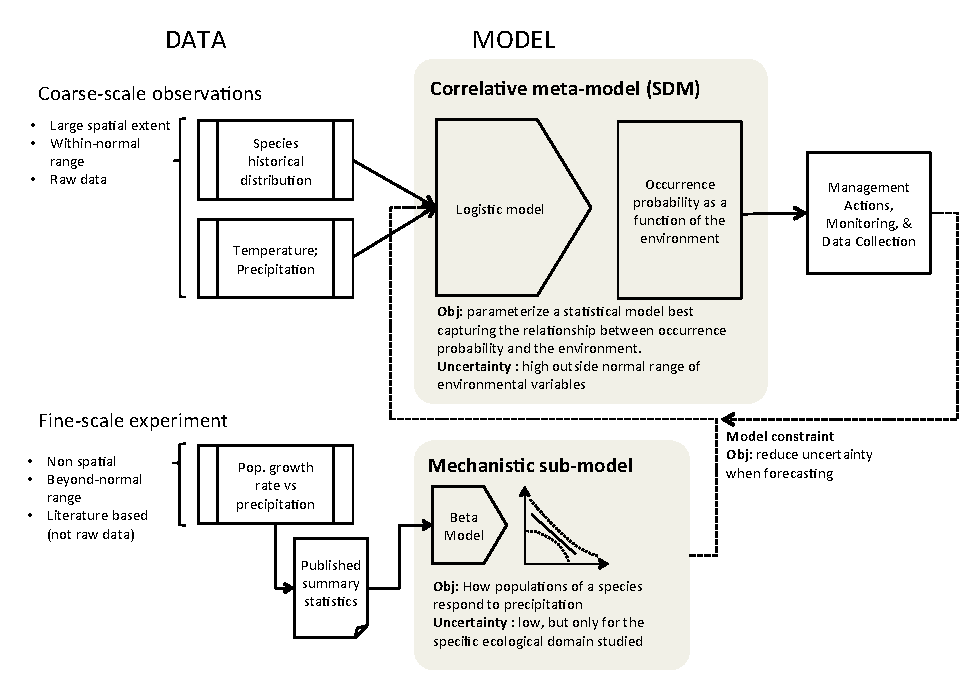
\includegraphics{figs/management.pdf}
	\caption{Sample workflow for applying the models presented in the first example in a management context.
	Critical steps include specifying the metamodel, identifying additional sources of information to be used as constraints on the metamodel, and using the integrated prediction for decision-making.
	As additional information becomes available from monitoring the results of management, this information can be incorporated in additional sub-models to further refine the metamodel.}
	\label{fig:management}
\end{figure}
%==================

In many cases, both the data and theory needed to apply our approach already exist, and all that is needed is the development of sub-models and their integration into a metamodel.
For example, climatic gradients may mediate competitive interactions \citep{Kunstler2011}, which means that simple correlative models that fail to account for competition may be wrong if the climate-competition association changes in the future.
In North America, the US Forest Service maintains a long term Forest Inventory Analysis database that could be utilized to parameterize a competition model.
Such a model need not explicitly predict occurrence limits; rather it could be integrated with a larger-scale model to include information about competition in a distribution model.
The phenological information needed to parameterize the sub-model for Example 2 is similarly available for a wide range of species \citep{Morin2009}.
There are also a number of networks collecting high-quality data with good temporal and spatial coverage (e.g., the National Ecological Observatory Network; NEON, and Long-Term Ecological Research sites; LTER).
There is great potential for these kinds of data to be used in fitting sub-models of the kind used in Example 1.
In other cases, qualitative model comparison efforts have already been made \citep{Morin2009, Cheaib2012}.
Our framework could be used \emph{post-hoc} on the outputs of these models to quantify uncertainty resulting from model disagreement.

%----------------------------
%----------------------------
%----------------------------

\subsection*{Challenges} 
Although our approach is highly flexible and can be applied in a number of situations, there are some challenges to successfully using the framework.
Data quality and availability can present a significant constraint on the number and type of models that can be implemented in our framework.
One obstacle is a lack of adequate and unbiased coverage of explanatory variables; exploratory analyses can be a significant aid in understanding how data coverage impacts resulting predictions \citep{Mckenney2002}.
Integration can solve these issues to some extent by using supplemental information (and conceptual advances) in additional sub-models where coverage is weak (e.g., Example 1, Figs. \ref{fig:ex1_precip}, \ref{fig:ex1_map}).
A strength of our approach is that it can be used without the full suite of data that would be required to run a fully mechanistic model. 
Given that the metamodel is correlative, it can be effectively implemented with, e.g., only presence-absence data, or, in the case where true absences are difficult to obtain, with presences and pseudo absences (provided sufficient care is used in interpreting the results of such a model).
Then any additional mechanistic data that are available will enhance predictions by constraining outputs of the metamodel. 

Determining the functions to use to express the likelihood of the sub-models given the metamodel (i.e., Eq. \ref{eq:ex1_integrated}) is a critical point.
The challenge is three fold: (1) which spatial and temporal scales (i.e. which processes), are to be considered, (2) how to build a scale the sub-models to be consistent with the metamodels, and (3) how error and uncertainty propagate from the sub-models to the metamodel. 
Although we argue that our proposed framework is able to easily deal with very different scales and that the Bayesian framework allows for an efficient integration of uncertainty throughout all scales considered, the building of scaling functions is an object of investigation on its own. 
It is likely that the modeling process may include multiple functions operating at different scales when taking all known processes and models into account. 
Indeed, if species distributions are a function of, e.g. population growth rate \citep{Guisan2000}, they will involve processes at the individual (e.g. competition) or cellular (e.g. photosynthesis) scales. 
Such very large differences in spatial scales would require more sophisticated upscaling methods than simple functions such as those we have used here. 
Our framework is still applicable whatever the chosen upscaling approach and is able to propagate uncertainties from sub-models to the metamodel.
\rev{Indeed, if a sub-model provides poor information (due, for example, to cross-scale nonlinearities in the response to the environment), the resulting metamodel predictions may be worse than the pre-integration naive model.
In general, we advise users of this framework to carefully consider the scaling in their models with respect to the biology of the organism studied, and to use prior model weights to downweight the scaled models when there is uncertainty about the applicability of a sub-model at the metamodel scale.
For instance, in the first example, we applied a model weight to decrease the influence of the mechanistic model on the metamodel (while still retaining some information contained therein), recognizing that such a simplistic model may not scale well.
Finally, as always when modelling ecological systems, we urge humility in the interpretation of model results and suggest the use of model evaluation and validation tools whenever possible.
We provide additional discussion on the implementation of model weights in Appendix S1.}

The implementation of the model itself can present an obstacle when model complexity increases. 
In many cases, off-the-shelf software can adequately express the model likelihoods with minimal programming, but more complicated models will require the development of custom programs. 
Developing such customized code would requires careful model specification, understanding of applied Bayesian methods, and, in some cases, extensive programming. 
However, the flexibility of our approach, and its transparency with respect to the propagation of uncertainty, will often outweigh the implementation challenges.

Finally, this approach is not just a new methodological tool but is a framework for forecasting species distributions which is fundamentally designed to make the link between modelers and practitioners while correctly estimating uncertainties and being updatable with new data and theoretical advances. 
A scientific approach such as presented here is particularly adapted to make a synthesis of available information and provide robust species distribution forecasts based on information known to be the best available scientific knowledge. 
It can incorporate large databases, valuing the efforts of data collection, and include models based on the latest theoretical advances, which is essential to decrease errors due to model specification \citep{Austin2007}. 
In addition, it provides practitioners and decision-makers with the best possible estimation of uncertainties, with direct applications to risk assessment or to guide the choice where investigating new research and accumulating new data. 
Finally, we argue that the adaptability of our approach is particularly appropriate in a world where collected data and theoretical knowledge is changing as quickly as climate and conservation practices must be adjusted accordingly.

\section*{Data Accessibility}
All data, as well as all code required to repeat the analyses, have been uploaded as online supporting information in Appendix S2.


%% ----------------------------------
%
%     Supporting information
%
%% ----------------------------------
\section*{Supporting information}
Appendix S1: Complete model description and model fitting details for the examples. \\
Appendix S2: Scripts and data required to reproduce the analyses.

\section*{Acknowledgements}
We acknowledge funding from the Quebec Centre for Biodiversity Science as well as NSERC strategic grant 430393-12. Comments from Charles Canham, William Godsoe, and Tamara Münkemüller improved a previous version of this manuscript. WT received support funding from the European Research Council under the European Community's Seven Framework Programme FP7/2007-2013 Grant Agreement no. 281422 (TEEMBIO). 

\nolinenumbers

%% ----------------------------------
%
%     REFERENCES
%
%% ----------------------------------

\renewcommand\refname{Literature Cited}
\bibliography{model_integration}{}
\bibliographystyle{model_integration}


%% ----------------------------------
%
%     BIOSKETCH (GEB)
%
%% ----------------------------------

%TC:break biosketch
\section*{Biosketch}
The Canada Research Chair in Biogeography and metacommunity ecology at the Université du Québec à Rimouski focuses on interactions between species distributions, community structure and ecosystem functioning.
We apply principles of spatial ecology to a variety of organisms and systems, from bacteria to entire forests.
We also use theoretical and simulation models to develop hypotheses and extend our work beyond the technical limitations of empirical studies.
More information can be found at: http://chaire-eec.uqar.ca/




\end{document}
